%%
%% The original source files were:
%%
%% examples_kmbeamer.dtx  (with options: `DarkConsole')
%% Copyright (c) 2011-2013 Kazuki Maeda <kmaeda@users.sourceforge.jp>
%% 
%% Distributable under the MIT License:
%% http://www.opensource.org/licenses/mit-license.php
%% 

\documentclass{beamer}
\usepackage{mathspec}
\usepackage{xeCJK}
\usepackage{graphicx}
\usepackage[figurename=Obraz]{caption}
\setCJKmainfont{IPAPMincho}
\setCJKsansfont{IPAGothic}
\setCJKmonofont{IPAGothic}

\setmainfont{FreeSerif}
\setsansfont{FreeSans}
\setmonofont{Latin Modern Mono}

\usetheme{DarkConsole}
\setbeamertemplate{theorems}[normal font]

\title{PROTOKÓŁ HTTP}
\subtitle{od 1.0 do 3.0}
\author{Jakub Sydor}
\date{16/01/2019}

\begin{document}

\begin{frame}
  \maketitle
\end{frame}

\begin{frame}{Spis treści}
  \tableofcontents
\end{frame}

\section{Wstęp}
\begin{frame}{Wstęp}
  Protokół HTTP został stworzony przez Tim Berners-Lee w roku 1989 jako standard komunikacji dla sieci World Wide Web.
  
  \vspace{1cm}
  
  Znajduje się na szczycie modelu ISO/OSI w warstwie Sesji.
  
  \vspace{1cm}
 
  Protokół HTTP definiuje, w jaki sposób zainicjować połączenie, jak wymieniać informację oraz zasoby i jak połączenie zakończyć.
\end{frame}

\section{Budowa zapytania}
\begin{frame}{Budowa zapytania}
    \begin{figure}[request]
    \caption{Przykładowe zapytanie do strony ms.polsl.pl/aktualnosci.php}
    \centering
    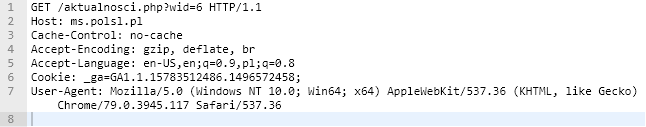
\includegraphics[width=\textwidth]{images/request.png}
    \end{figure}
    \vspace{1pt}
    \begin{center}
        \begin{Huge}
            +
        \end{Huge}
    \end{center}
    \begin{center}
        Ciało zapytania (o ile istnieje)
    \end{center}
\end{frame}

\section{Budowa odpowiedzi}
\begin{frame}{Budowa odpowiedzi}
    \begin{figure}[request]
        \caption{Przykładowa odpowiedź ze strony ms.polsl.pl/aktualnosci.php}
        \centering
        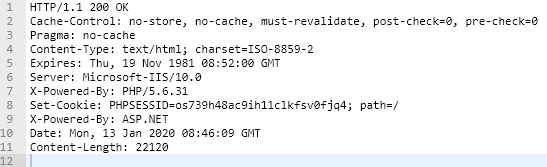
\includegraphics[width=\textwidth]{images/response.png}
    \end{figure}
    \vspace{1pt}
    \begin{center}
        \begin{Huge}
            +
        \end{Huge}
    \end{center}
    \begin{center}
        Ciało odpowiedzi (o ile istnieje)
    \end{center}
\end{frame}

\section{HTTP/1.1}
\begin{frame}{HTTP/1.1}
    \begin{center}
        \begin{Huge}
           Komunikacja w HTTP/1.1
        \end{Huge}
    \end{center}
\end{frame}

\begin{frame}{Przebieg komunikacji w HTTP/1.1}
    \begin{enumerate}
        \item Wysłanie żądanie do serwera DNS
        \item Odpowiedź serwera DNS
        \item Rozpoczęcie połączenia TCP z serwerem (wymiana pakietów SYN/ACK)
        \item Wysłanie żądania HTTP do serwera
        \item Odebrania danych od serwera
    \end{enumerate}
    
    \pause
    
    \vspace{15pt}
    
    \begin{large}
    Sposób przesyłu:
    \end{large}
    \begin{itemize}
        \item Przesyłamy żądania jako PLAINTEXT
        \item Nagłówki oraz ciało wysyłane są razem
        \item Wiele połączeń lub użycie HTTP pipelining
        \item Kolejkowanie zapytań
    \end{itemize}
\end{frame}

\section{HTTP/2}
\begin{frame}{HTTP/2}
    \begin{center}
        \begin{Huge}
           Komunikacja w HTTP/2
        \end{Huge}
    \end{center}
\end{frame}

\begin{frame}{Przebieg komunikacji w HTTP/2}
    \begin{enumerate}
        \item Wysłanie żądanie do serwera DNS
        \item Odpowiedź serwera DNS
        \item Rozpoczęcie połączenia TCP z serwerem (wymiana pakietów SYN/ACK)
        \item Ustanowienie bezpiecznego połączenia (TLS handshake)
        \item Wysłanie żądania HTTP do serwera
        \item Odebrania danych od serwera
    \end{enumerate}
    
    \pause
    
    \vspace{15pt}
    
    \begin{large}
    Sposób przesyłu:
    \end{large}
    \begin{itemize}
        \item Przesyłamy żądania w formie binarnej za pomocą strumieni (NOWOŚĆ)
        \item Nagłówki oraz ciało wysyłane są w osobnych strumieniach (NOWOŚĆ)
        \item Jedno połączenie oraz priorytety (NOWOŚĆ)
    \end{itemize}
\end{frame}

\section{HTTP/3}
\begin{frame}{HTTP/3}
    \begin{center}
        \begin{Huge}
           Komunikacja w HTTP/3
        \end{Huge}
    \end{center}
\end{frame}

\begin{frame}{Przebieg komunikacji w HTTP/3}
    \begin{enumerate}
        \item Wysłanie żądanie do serwera DNS
        \item Odpowiedź serwera DNS
        \item Rozpoczęcie połączenia za pomocą protokołu QUIC
        \item Ustanowienie bezpiecznego połączenia (Zaimplementowane w QUIC)
        \item Wysłanie żądania HTTP do serwera
        \item Odebrania danych od serwera
    \end{enumerate}
\end{frame}

\subsection{QUIC}
\begin{frame}{Protokół QUIC}
    QUIC(Quick UDP Internet Connection) jest to protokół warstwy transportowej, wymagający szyfrowania. Został stworzony w Google, aby uczynić HTTP wydajniejszym oraz bezpieczniejszym. Działa pod kontrolą UDP.
    
    \vspace{20pt}
    \begin{large}
    Zalety:
    \end{large}
    \begin{itemize}
        \item Szybsze nawiązanie połączenia
        \item Lepsze obsługa utraty pakietów i/lub zmiany sieci
        \item Większe możliwości implementacji
    \end{itemize}
    
    \pause
    
    \begin{large}
    Wady:
    \end{large}
    \begin{itemize}
        \item Połączenie bardziej obciąża komputer
        \item Trudniejsze debugowanie
    \end{itemize}
    
\end{frame}

\end{document}
\endinput
